\section{爆破}\label{sec:blow-ups}

本节通过例子介绍爆破, 这一构造在代数几何中有许多应用. 在各个例子中, 我们着重说明一种特定应用: 用爆破消解奇点. 先从一种非常具体的爆破开始: $\mathbb{A}^{n}$ 在 $0$ 处的爆破. 为便于理解记号, 始终用 $x_{1},\ldots,x_{n}$ 表示 $\mathbb{A}^{n}$ 的坐标, 用 $y_{1},\ldots,y_{n}$ 表示 $\mathbb{P}^{n-1}$ 的齐次坐标 (注意从 $y_{1}$ 开始, 而不是 $y_{0}$).

\begin{Definition}{仿射空间在原点的爆破}\leavevmode\label{def:blowup-of-affine-space-at-origin}
$\mathbb{A}^{n}$ \emph{在原点的爆破}是拟射影簇
\[
  \operatorname{Bl}_{0}(\mathbb{A}^{n})
   =\mathcal{V}(x_{i}y_{j}-x_{j}y_{i}\mid1\le i<j\le n)
    \subseteq\mathbb{A}^{n}\times\mathbb{P}^{n-1},
\]
并配有\emph{爆破映射} $\pi:\operatorname{Bl}_{0}(\mathbb{A}^{n})\to\mathbb{A}^{n}$, 它是 $\mathbb{A}^{n}\times\mathbb{P}^{n-1}$ 到第一因子的投影的限制.
\end{Definition}

在深入探究定义的细节之前, 先用第一个非平凡的情形 $n=2$ 说明它.

\begin{Example}{$\mathbb{A}^{2}$ 在原点的爆破}\leavevmode\label{ex:blowup-of-affine-plane-at-origin}
\BookPairedFigure{
考察 $\mathbb{A}^{2}$ 在原点的爆破,
\[
  \operatorname{Bl}_{0}(\mathbb{A}^{2})
  =\mathcal{V}(x_{1}y_{2}-x_{2}y_{1})\subseteq\mathbb{A}^{2}\times\mathbb{P}^{1}.
\]
右图给出了它在 $\mathbb{R}$ 上的情形, 以及 (向下的) 爆破映射
\[
  \pi:\operatorname{Bl}_{0}(\mathbb{A}^{2})\to\mathbb{A}^{2}.
\]
为理解爆破的这个图示, 考察一点
\[
  \bigl((a_{1},a_{2}),[b_{1},b_{2}]\bigr)\in\operatorname{Bl}_{0}(\mathbb{A}^{2}).
\]
}{
\phantomsection\label{fig:blowup-of-affine-plane}%
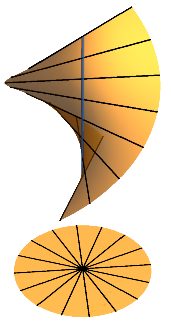
\includegraphics[width=.79\linewidth]{figures/blowup-of-affine-plane.pdf}
}
按定义, 必有 $a_{1}b_{2}=a_{2}b_{1}$. 稍加思考可知, 这等价于 $(a_{1},a_{2})\in\mathbb{A}^{2}$ 位于由 $b=[b_{1}:b_{2}]\in\mathbb{P}^{1}$ 确定的直线上. 换句话说, $\operatorname{Bl}_{0}(\mathbb{A}^{2})$ 中 $\mathbb{P}^{1}$ 坐标固定为 $b$ 的点, 与 $\mathbb{A}^{2}$ 中由点 $b\in\mathbb{P}^{1}$ 参数化的直线上的点有典范对应.

因此在上图中, 我们将 $\mathbb{P}^{1}$ 画作竖直坐标. 此时, $\mathbb{A}^{2}$ 中的每条直线都提升为 $\operatorname{Bl}_{0}(\mathbb{A}^{2})\subseteq\mathbb{A}^{2}\times\mathbb{P}^{1}$ 中同一条直线, 位于该直线所确定的 $\mathbb{P}^{1}$ 坐标的高度. 不过, 这幅图并不完整: 要补全它, 应把 $\operatorname{Bl}_{0}(\mathbb{A}^{2})$ 的顶部绕回来接到底部, 形成一条 Möbius 带, 因为当我们把直线绕原点旋转时, 最终会回到出发处.

注意, 除原点外, $\mathbb{A}^{2}$ 中每一点在 $\operatorname{Bl}_{0}(\mathbb{A}^{2})$ 中都有唯一原像. 这只是说, 这些点中的每一个都确定唯一一条经过原点的直线. 而原点的原像由整个 $\mathbb{P}^{1}$ 构成, 它参数化 $\mathbb{A}^{2}$ 中过原点的所有直线. 换句话说, 在原点对 $\mathbb{A}^{2}$ 作\textquotedbl{}爆破\textquotedbl{}, 可以视为用射影空间 $\mathbb{P}^{1}$ 的一个副本替换 $\mathbb{A}^{2}$ 中的原点.
\end{Example}

\BookPairedNote{
前一例中对 $\operatorname{Bl}_{0}(\mathbb{A}^{2})$ 建立的直观理解, 很自然地推广到 $\operatorname{Bl}_{0}(\mathbb{A}^{n})$. 特别地, 点 $(a,b)\in\mathbb{A}^{n}\times\mathbb{P}^{n-1}$ 在 $\operatorname{Bl}_{0}(\mathbb{A}^{n})$ 上, 当且仅当 $a\in\mathbb{A}^{n}$ 在由 $b\in\mathbb{P}^{n-1}$ 确定的过原点的直线上 (Exercise~\ref{ex:blowup-incidence-condition-is-line-membership}).
}{
\textquotedbl{}爆破\textquotedbl{}这个术语, 最好把它理解为给气球充气或放大图像的比喻, 而不是爆炸的比喻.
}
特别地, 可以把 $\operatorname{Bl}_{0}(\mathbb{A}^{n})$ 看成用整个射影空间 $\mathbb{P}^{n-1}$ 替换 $\mathbb{A}^{n}$ 的原点的结果. 该射影空间参数化所有可能沿着趋近原点的切方向. 除了这一爆破的直观描述, 还应注意 $\operatorname{Bl}_{0}(\mathbb{A}^{n})$ 不可约, 维数为 $n$, 并且光滑 (Exercise~\ref{ex:irreducibility-dimension-and-smoothness-of-affine-space-blowup}).

已经描述 $\mathbb{A}^{n}$ 在原点的爆破, 现在可以定义仿射簇 $X\subseteq\mathbb{A}^{n}$ 在原点的爆破.

\begin{Definition}{仿射簇在原点的爆破}\leavevmode\label{def:blowup-of-affine-variety-at-origin}
令 $X\subseteq\mathbb{A}^{n}$ 为包含原点的 Zariski 闭集. $X$ \emph{在原点的爆破}是拟射影簇
\[
  \operatorname{Bl}_{0}(X)=\overline{\pi^{-1}(X\setminus\{0\})}
    \subseteq\operatorname{Bl}_{0}(\mathbb{A}^{n}).
\]
\end{Definition}

换句话说, 为计算 $X\subseteq\mathbb{A}^{n}$ 在原点的爆破, 先去掉原点, 在 $\operatorname{Bl}_{0}(\mathbb{A}^{n})$ 中考察 $X\setminus\{0\}$ 的原像, 再取 Zariski 闭包. 为获得直观认识, 来看一个具体例子.

\begin{Example}{$\mathbb{A}^{2}$ 中结点曲线的爆破}\leavevmode\label{ex:blowup-of-nodal-affine-curve}
\BookPairedFigure{
考察仿射曲线
\[
  X=\mathcal{V}(x_{1}^{2}+x_{1}^{3}-x_{2}^{2})\subseteq\mathbb{A}^{2},
\]
右侧下图描绘了这条曲线, 上图描绘了它的爆破 $\operatorname{Bl}_{0}(X)$. 为说明 $\operatorname{Bl}_{0}(X)$ 的这一图示, 首先注意 (Exercise~\ref{ex:parametrize-nodal-affine-curve}) 可以把 $X$ 参数化为
\[
  X=\{(a^{2}-1,a^{3}-a)\mid a\in\mathbb{A}^{1}\},
\]
其中 $a=1$ 和 $a=-1$ 都对应原点, $X$ 在这里绕回并与自身相交.
}{
\phantomsection\label{fig:blowup-of-nodal-curve}%
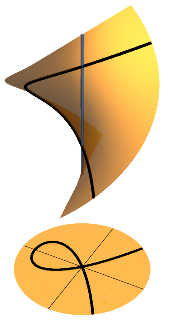
\includegraphics[width=.79\linewidth]{figures/blowup-of-nodal-curve.pdf}
}
由于对所有 $a\ne\pm1$ 有 $[a^{2}-1:a^{3}-a]=[1:a]$, 可推出
\[
  \pi^{-1}(X\setminus\{0\})
  =\{\bigl((a^{2}-1,a^{3}-a),[1:a]\bigr)\mid a\in\mathbb{A}^{1}\setminus\{\pm1\}\}
  \subseteq\mathbb{A}^{2}\times\mathbb{P}^{1}.
\]
为计算 $\pi^{-1}(X\setminus\{0\})$ 的闭包, 只需在上式中补上缺少的两个取值 $a=\pm1$ (Exercise~\ref{ex:closure-and-smoothness-of-nodal-curve-blowup}), 得
\[
  \operatorname{Bl}_{0}(X)=
  \{\bigl((a^{2}-1,a^{3}-a),[1:a]\bigr)\mid a\in\mathbb{A}^{1}\}.
\]
注意原点在 $\operatorname{Bl}_{0}(X)$ 中的原像包含两点 $[1:\pm1]$, 对应 $\mathbb{A}^{2}$ 中斜率为 $\pm1$ 的直线, 它们可视为 $X$ 的两个\textquotedbl{}分支\textquotedbl{}在原点的切线. 因此, 在原点对 $X$ 作爆破, 就按两个分支的斜率把自交点分开了.
\end{Example}

Example~\ref{ex:blowup-of-nodal-affine-curve} 的曲线 $X$ 在原点奇异, 用 Jacobian 判据很容易验证. 但其爆破 $\operatorname{Bl}_{0}(X)$ 同构于 $\mathbb{A}^{1}$ (Exercise~\ref{ex:closure-and-smoothness-of-nodal-curve-blowup}), 所以爆破是光滑的. 换句话说, 爆破\emph{消解}了 $X$ 中的奇点. 更一般地, 拟射影簇 $X$ 的一个\emph{奇点消解}是一个光滑拟射影簇 $Y$ 和一个正则映射 $\pi:Y\to X$, 该映射在 $X$ 的光滑部分的原像上限制为同构. (特别地, 这意味着 $X$ 与 $Y$ 双有理.) 爆破是构造奇点消解的一个重要工具. 下一例进一步说明如何用一次爆破消解曲线的奇点.

\begin{Example}{$\mathbb{A}^{2}$ 中尖点曲线的爆破}\leavevmode\label{ex:blowup-of-cuspidal-affine-curve}
\BookPairedFigure{
考察仿射曲线
\[
  X=\mathcal{V}(x_{1}^{2}-x_{2}^{3})\subseteq\mathbb{A}^{2},
\]
右侧下图描绘了这条曲线, 上图描绘了它的爆破 $\operatorname{Bl}_{0}(X)$. 和前一例一样, 考察 $X$ 的一个参数化:
\[
  X=\{(a^{3},a^{2})\mid a\in\mathbb{A}^{1}\},
\]
其中 $a=0$ 对应原点处的奇点. 对所有 $a\ne0$ 有 $[a^{3}:a^{2}]=[a:1]$.
}{
\phantomsection\label{fig:blowup-of-cuspidal-curve}%
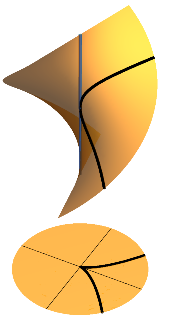
\includegraphics[width=.79\linewidth]{figures/blowup-of-cuspidal-curve.pdf}
}
因此
\[
  \pi^{-1}(X\setminus\{0\})
  =\{\bigl((a^{3},a^{2}),[a:1]\bigr)\mid a\in\mathbb{A}^{1}\setminus\{0\}\}
  \subseteq\mathbb{A}^{2}\times\mathbb{P}^{1}.
\]
和前一例作类似的论证, 在上式中补上取值 $a=0$ 即可算出闭包, 得
\[
  \operatorname{Bl}_{0}(X)=\{\bigl((a^{3},a^{2}),[a:1]\bigr)\mid a\in\mathbb{A}^{1}\}.
\]
和前一例一样, 有 $\operatorname{Bl}_{0}(X)\cong\mathbb{A}^{1}$. 因此再次看到, 爆破 $\operatorname{Bl}_{0}(X)$ 是 $X$ 中尖点奇性的一个消解. 直观地说, 爆破使我们能够用较高维空间中的一条光滑路径来替换 $X$ 在原点处方向的急剧改变.
\end{Example}

到目前为止只看了 $\mathbb{A}^{2}$ 中曲线的爆破. 把维数提高一维, 现在考察 $\mathbb{A}^{3}$ 中曲面的爆破.

\begin{Example}{仿射锥的爆破}\leavevmode\label{ex:blowup-of-affine-cone}
\BookPairedFigure{
考察仿射曲面
\[
  X=\mathcal{V}(x_{1}^{2}+x_{2}^{2}-x_{3}^{2})\subseteq\mathbb{A}^{3}.
\]
在 $\mathbb{R}$ 上, 这是以原点为顶点的圆锥, 如右侧下图所示. 爆破 $\operatorname{Bl}_{0}(X)$ 如上图所示. 为直观理解这里发生了什么, 注意 $X$ 是 $\mathbb{A}^{3}$ 中许多直线的并, 它们都在原点相交. 在原点作爆破, 会把相交的所有这些直线分开, 从而可以把 $\operatorname{Bl}_{0}(X)$ 视为 $\mathbb{A}^{3}\times\mathbb{P}^{2}$ 中这些直线的 (爆破的) \emph{不交}并.
}{
\phantomsection\label{fig:blowup-of-affine-cone}%
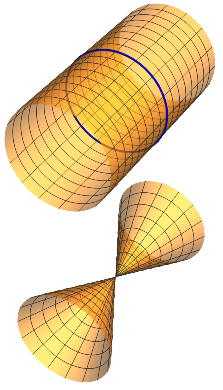
\includegraphics[width=\linewidth]{figures/blowup-of-affine-cone.pdf}
}
在 $\mathbb{R}$ 上工作时, 这些直线的 (爆破的) 不交并可以自然地与上图中的圆柱等同. 不过提醒读者, 在 $\mathbb{C}$ 这样的代数闭域上工作时, $\operatorname{Bl}_{0}(X)$ 的整体几何并没有这么直接.
\end{Example}

本节的例子只是略微触及爆破理论的丰富内容. 有一种更一般的 (内在的) 构造 $\operatorname{Bl}_{Y}(X)$, 沿拟射影簇 $X$ 的一个闭子簇 $Y$ 作爆破. 直观地说, 可通过用参数化该点处法向于 $Y$ 的切方向的射影空间替换 $Y$ 的每一点, 从 $X$ 构造 $\operatorname{Bl}_{Y}(X)$. 爆破理论中最著名的结果是日本数学家 Heisuke Hironaka 在 1964 年证明的奇点消解定理. 它说, 特征零的代数闭域上的每个拟射影簇, 都可以通过一系列爆破消解为光滑簇. 在本节讨论的消解例子中, 消解奇点都只需要一次爆破. 要看必须用两次爆破才能消解的曲线奇点, 请见 Exercise~\ref{ex:two-blowups-resolve-higher-cusp}. 在正特征下, 是否每个簇都能消解仍是一个未解决的问题.

\BookExerciseHeading
\begin{BookExercises}
  \item\label{ex:blowup-incidence-condition-is-line-membership} 证明点 $(a,b)\in\mathbb{A}^{n}\times\mathbb{P}^{n-1}$ 在 $\operatorname{Bl}_{0}(\mathbb{A}^{n})$ 上, 当且仅当 $a$ 在由点 $b\in\mathbb{P}^{n-1}$ 确定的 $\mathbb{A}^{n}$ 中的直线上.
  \item\label{ex:fibres-of-blowup-of-affine-space-at-origin} 考察爆破映射 $\pi:\operatorname{Bl}_{0}(\mathbb{A}^{n})\to\mathbb{A}^{n}$.
  \begin{enumerate}
    \item 证明若点 $(a_{1},\ldots,a_{n})\in\mathbb{A}^{n}$ 的坐标 $a_{i}$ 中至少有一个非零, 则该点的原像为单点.
    \item 证明原点的原像同构于 $\mathbb{P}^{n-1}$.
  \end{enumerate}
  \item\label{ex:irreducibility-dimension-and-smoothness-of-affine-space-blowup}
  \begin{enumerate}
    \item 证明 $\operatorname{Bl}_{0}(\mathbb{A}^{n})$ 有一个同构于 $\mathbb{A}^{n}\setminus\{0\}$ 的稠密开子集.
    \item 证明 $\operatorname{Bl}_{0}(\mathbb{A}^{n})$ 不可约.
    \item 证明 $\operatorname{Bl}_{0}(\mathbb{A}^{n})$ 的维数是 $n$.
    \item 证明 $\operatorname{Bl}_{0}(\mathbb{A}^{n})$ 光滑.
  \end{enumerate}
  \item\label{ex:parametrize-nodal-affine-curve} 令 $X=\mathcal{V}(x_{1}^{2}+x_{1}^{3}-x_{2}^{2})\subseteq\mathbb{A}^{2}$. 证明
  \[
    X=\{(a^{2}-1,a^{3}-a)\mid a\in\mathbb{A}^{1}\}.
  \]
  \item\label{ex:closure-and-smoothness-of-nodal-curve-blowup} 考察子集
  \[
    Y=\{\bigl((a^{2}-1,a^{3}-a),[1:a]\bigr)\mid a\in\mathbb{A}^{1}\setminus\{\pm1\}\}
    \subseteq\mathbb{A}^{2}\times\mathbb{P}^{1}.
  \]
  \begin{enumerate}
    \item 设 $f\in K[x_{1},x_{2},y_{1},y_{2}]$ 在 $Y$ 的每一点处消没. 证明 $f$ 也在两点 $\bigl((0,0),[1:\pm1]\bigr)$ 处消没.
    \item 找出三个多项式 $f_{1},f_{2},f_{3}\in K[x_{1},x_{2},y_{1},y_{2}]$, 使
    \[
      \mathcal{V}(f_{1},f_{2},f_{3})
      =\{\bigl((a^{2}-1,a^{3}-a),[1:a]\bigr)\mid a\in\mathbb{A}^{1}\}
        \subseteq\mathbb{A}^{2}\times\mathbb{P}^{1}.
    \]
    \item 推出
    \[
      \overline{Y}=\{\bigl((a^{2}-1,a^{3}-a),[1:a]\bigr)\mid a\in\mathbb{A}^{1}\}.
    \]
    \item 证明 $\overline{Y}\cong\mathbb{A}^{1}$.
  \end{enumerate}
  \item\label{ex:two-blowups-resolve-higher-cusp} 令 $X=\mathcal{V}(x_{1}^{2}-x_{2}^{5})\subseteq\mathbb{A}^{2}$. 本题说明必须对 $X$ 作两次爆破才能消解其奇点.
  \begin{enumerate}
    \item 证明 $X$ 在原点奇异, 而在其他各点光滑.
    \item 证明 $\operatorname{Bl}_{0}(X)\subseteq\mathbb{A}^{2}\times\mathbb{P}^{1}$ 在点 $\bigl((0,0),[0:1]\bigr)$ 处奇异.
    \item 令 $U\subseteq\mathbb{A}^{2}\times\mathbb{P}^{1}$ 为 $y_{2}\ne0$ 的仿射开子集, 置 $Y=U\cap\operatorname{Bl}_{0}(X)$. 则 $Y$ 为 $\operatorname{Bl}_{0}(X)$ 的仿射开子集, 在 $U\cong\mathbb{A}^{3}$ 的原点处有奇点. 证明 $\operatorname{Bl}_{0}(Y)$ 光滑.
  \end{enumerate}
  \item\label{ex:blowup-extends-direction-map-to-regular-map} 考察由下式给出的有理映射 $F:\mathbb{A}^{n}\mathrel{\rightdasharrow}\mathbb{P}^{n-1}$:
  \[
    F(a_{1},\ldots,a_{n})=[a_{1}:\cdots:a_{n}],
  \]
  它在 $\mathbb{A}^{n}\setminus\{(0,\ldots,0)\}$ 上正则.
  \begin{enumerate}
    \item 证明不存在正则映射 $\widetilde{F}:\mathbb{A}^{n}\to\mathbb{P}^{n-1}$ 在 $\mathbb{A}^{n}\setminus\{(0,\ldots,0)\}$ 上与 $F$ 一致.
    \item 构造正则映射 $G:\operatorname{Bl}_{0}(\mathbb{A}^{n})\to\mathbb{P}^{n-1}$, 使对所有满足 $a\ne(0,\ldots,0)$ 的 $(a,b)\in\operatorname{Bl}_{0}(\mathbb{A}^{n})$ 有 $G(a,b)=F(a)$.
  \end{enumerate}
  本题说明爆破的另一种应用: 对有理映射的定义域作爆破, 往往可以用一个与它双有理的定义域替换原定义域, 使有理映射能够延拓为正则映射.
\end{BookExercises}
